\documentclass[12pt]{eDA_conquer2026}
\addbibresource{references.bib}

% Title ---------------------------------------------------------------------
\title{%
  \begin{center}
        \Large {AI VIET NAM -- eDA Conquer 2026}\\[.5ex]
        \Huge \textbf{Phân tích danh mục tín dụng KHDN -- AIV Bank}\\[.5ex] % TODO: tên bài tạm, nhóm chốt lại
  \end{center}
}

% Author --------------------------------------------------------------------
\posttitle{
\author{
\begin{minipage}{\textwidth}
\centering
{
\vspace{-1.5em}
\textbf{Nhóm Datalyst:} Nguyễn Minh Việt, Trần Thị Khánh Huyền, Ngô Nguyễn Huy Khương, Lê Quốc Hùng, Nguyễn Duy Kiên
}\
\end{minipage}
}
}
\date{}

% Header --------------------------------------------------------------------
\pagestyle{fancy}
\fancyhf{}
\lhead{\href{https://www.facebook.com/aivietnam.edu.vn}{\textcolor{aivnGreen}{\bfseries AI VIET NAM (eDA Conquer 2026)}}}
\rhead{\href{https://aivietnam.edu.vn/}{\textcolor{aivnGreen}{\bfseries aivietnam.edu.vn}}}
\fancyfoot[C]{\thepage}
\renewcommand{\headrulewidth}{1.0pt}
\renewcommand{\headrule}{{\color{aivnGreen}\hrule width\headwidth height\headrulewidth \vskip-\headrulewidth}}

\begin{document}
\maketitle
\vspace{-3em}

\section*{Tóm tắt cho lãnh đạo Khối KHDN}
\addcontentsline{toc}{section}{Tóm tắt cho lãnh đạo Khối KHDN}

\begin{aivncodebox}[Kết luận chính tại 30/06/2026]
Dư nợ AIV Bank đạt 98.367,3 tỷ đồng, tăng 1,25\% so với tháng trước và 10,95\% so với cùng kỳ năm trước. Dư nợ OD3-5 tăng 37,8\% so với cùng tháng năm trước, nhanh hơn quy mô danh mục. Tỷ lệ OD3-5 là 2,63\%, tăng 0,25 điểm phần trăm so với cuối tháng trước, nhưng mức tăng này đến từ một hợp đồng 390 tỷ đồng. Khi loại hợp đồng đó, tỷ lệ là 2,24\%, thấp hơn cuối tháng trước 0,14 điểm phần trăm.
\smallskip

Dư nợ OD2 giảm 31,6\%, nhưng trong số dư nợ rời OD2 chỉ 42\% trở về nhóm 1 và 51\% chuyển sang OD3, nên mức giảm này chưa cho thấy chất lượng tín dụng cải thiện. Micro và Small tạo 50,2\% NII YTD, trong khi MICRO cũng chiếm 23,6\% dư nợ OD3-5 so với 20,20\% tổng dư nợ.
\smallskip

\textbf{Đề xuất ưu tiên.} (1) Lập danh sách theo dõi các khoản lớn đang ở OD2 hoặc quá hạn từ 60 ngày, bắt đầu từ hợp đồng AIV-LN-0007842. (2) Báo cáo tỷ lệ OD3-5 kèm tỷ lệ khi loại khoản lớn nhất. (3) Theo dõi hằng tháng dòng chuyển nhóm từ OD2 sang OD3, cùng NIM và tỷ lệ OD3-5 theo phân khúc.
\smallskip

\textbf{Giới hạn chính.} Dữ liệu chỉ có số dư cuối tháng và dòng chuyển nhóm mới phản ánh một tháng, nên chưa đủ để kết luận xu hướng hay nguyên nhân nghiệp vụ.
\end{aivncodebox}

\newpage
\setcounter{tocdepth}{1}
\tableofcontents
\thispagestyle{fancy}
\vspace{0.6cm}

\newpage
\section*{Thuật ngữ dùng trong báo cáo}
\addcontentsline{toc}{section}{Thuật ngữ dùng trong báo cáo}
\begin{table}[H]
\centering
\renewcommand{\arraystretch}{1.3}
\begin{tabularx}{\linewidth}{@{} >{\bfseries}p{4.5cm} X @{}}
\toprule
Thuật ngữ & Ý nghĩa \\
\midrule
Dư nợ cuối kỳ (EOP) & Tổng số dư nợ gốc tại một ngày chốt cuối tháng. \\
DNBQ YTD & Dư nợ bình quân lũy kế từ đầu năm đến thời điểm báo cáo. \\
NII (Net Interest Income) & Thu nhập lãi thuần từ hoạt động tín dụng. \\
TOI (Total Operating Income) & Tổng thu nhập hoạt động (bao gồm NII và thu nhập ngoài lãi). \\
MoM (Month-over-Month) & Tỷ lệ thay đổi so với tháng liền trước. \\
YoY (Year-over-Year) & Tỷ lệ thay đổi so với cùng kỳ năm trước. \\
OD2 (Overdue 2) & Dư nợ nhóm 2 (Nợ cần chú ý). \\
OD3-5 & Dư nợ từ nhóm 3 đến nhóm 5 (Nợ xấu). \\
Nhóm 1 & Nợ đủ tiêu chuẩn (nhóm nợ thấp nhất, không có dấu hiệu rủi ro). \\
Dòng chuyển nhóm & Phần dư nợ dịch chuyển giữa các nhóm nợ giữa hai mốc 31/05 và 30/06/2026. \\
ĐVKD & Đơn vị kinh doanh (Chi nhánh, Trung tâm KHDN). \\
\bottomrule
\end{tabularx}
\end{table}

\section{Vấn đề và câu hỏi phân tích}

Doanh nghiệp trong bài là ngân hàng AIV Bank. Ban lãnh đạo khối Khách hàng Doanh nghiệp cần theo dõi tình hình ngân hàng hiện tại thông qua 3 câu hỏi trọng tâm sau:

\vspace{0.2cm}
\noindent \textbf{Q1.} Dư nợ hiện tại là bao nhiêu và có biến động ra sao?

\noindent \textbf{Q2.} Danh mục cho vay nào đang tạo ra mức thu nhập?

\noindent \textbf{Q3.} Những khoản vay nào đang có dấu hiệu rủi ro và tiềm ẩn nguy cơ mất vốn?

\vspace{0.2cm}
Để làm rõ và bổ sung ý nghĩa cho 3 vấn đề trọng tâm trên, ta cần phân tích để tìm ra câu trả lời cho các câu hỏi chi tiết sau:

\vspace{0.2cm}
\noindent \textbf{Đối với Q1 (Dư nợ và biến động):} Câu hỏi được tách thành ba nhánh để đánh giá toàn diện quy mô, nguồn gốc tăng trưởng và mức độ tập trung:
\begin{itemize}[label=--, leftmargin=0.8cm, itemsep=0.2em]
    \item Dư nợ cuối kỳ và DNBQ YTD hiện ở mức nào; thay đổi ra sao so với tháng trước và cùng kỳ năm trước?
    \item Mức tăng/giảm dư nợ đến từ kỳ hạn, phân khúc, ngành, sản phẩm và ĐVKD nào? Trọng tâm là giá trị tăng tuyệt đối, không chỉ tỷ lệ tăng trưởng?
    \item Top 10 ngành và Top 10 ĐVKD đang chiếm bao nhiêu tổng dư nợ; mức tập trung thay đổi như thế nào qua thời gian?
\end{itemize}

\vspace{0.2cm}
\noindent \textbf{Đối với Q2 (Thu nhập từ danh mục):} Việc tập trung vào ba câu hỏi này giúp đo lường hiệu quả sinh lời thực tế, kiểm tra chất lượng tăng trưởng tín dụng và xác định nguồn gốc lợi nhuận:
\begin{itemize}[label=--, leftmargin=0.8cm, itemsep=0.2em]
    \item Giá trị NII, TOI YTD là bao nhiêu so với cùng kỳ tháng trước? \textit{(Nhằm xác định nguồn thu chính và xu hướng lợi nhuận cốt lõi từ việc cho vay).}
    \item Mức tăng thu nhập có tương xứng với mức tăng dư nợ không? \textit{(Nhằm đảm bảo ngân hàng không hy sinh biên lợi nhuận/chấp nhận rủi ro cao chỉ để đổi lấy quy mô dư nợ).}
    \item Phân khúc, đơn vị kinh doanh (ĐVKD) hay nhóm khách hàng nào đang đóng góp trọng yếu vào tổng thu nhập? \textit{(Nhằm xác định động lực chính tạo ra lợi nhuận lớn nhất và đánh giá mức độ rủi ro khi nguồn thu bị tập trung quá mức).}
\end{itemize}

\vspace{0.2cm}
\noindent \textbf{Đối với Q3 (Khoản vay có dấu hiệu rủi ro):} Việc đi sâu vào các thành phần nợ xấu giúp kiểm soát nguồn phát sinh chi phí dự phòng và đánh giá chất lượng tín dụng thực chất:
\begin{itemize}[label=--, leftmargin=0.8cm, itemsep=0.2em]
    \item Tỷ lệ OD2 và OD3-5 hiện tại là bao nhiêu, và đã thay đổi bao nhiêu điểm phần trăm so với cuối tháng trước và cùng tháng năm trước?
    \item Rủi ro tập trung ở ngành, đơn vị kinh doanh (ĐVKD) và phân khúc nào?
    \item Khi dư nợ OD2 giảm, phần giảm đến từ khoản vay trở về nhóm 1 hay từ khoản vay chuyển sang nhóm nợ xấu hơn?
\end{itemize}

\vspace{0.2cm}
Dư nợ OD2 (nợ nhóm 2) và OD3-5 (nợ nhóm 3 đến 5, còn gọi là nợ xấu) chiếm tỷ trọng nhỏ trong tổng dư nợ, nhưng là nguồn phát sinh chi phí dự phòng. Nếu dư nợ OD2 giảm do khoản vay chuyển sang nhóm nợ xấu hơn, mức giảm đó không phản ánh chất lượng tín dụng cải thiện, và nguồn lực xử lý nợ có thể bị đặt vào đối tượng chưa cần ưu tiên.

\section{Dữ liệu và cách chuẩn bị}

Dataset AIV Bank là dữ liệu giả lập theo mô hình star schema, phục vụ Khối KHDN. Dữ liệu có 10.000 khách hàng, 31.104 hợp đồng và 333.882 dòng \textit{fact\_loan\_balance}. Bảng số dư gồm 31 ngày chốt cuối tháng, từ 31/12/2023 đến 30/06/2026. Đơn vị tiền tệ trong phân tích là VND sau quy đổi. Các bảng chính sử dụng gồm \textit{fact\_loan\_balance}, \textit{fact\_income\_monthly}, \textit{dim\_loan\_contract}, \textit{dim\_customer}, \textit{dim\_branch}, \textit{dim\_segment}, \textit{dim\_industry}, \textit{dim\_product} và \textit{dim\_date}. Dataset được cung cấp ở trạng thái sạch. Theo báo cáo QC, các quan hệ FK hợp lệ, không có dòng số dư không dương, không có duplicate khóa fact và không có NULL ở các bảng chính. Ký hiệu $B_t$ là tổng dư nợ cuối kỳ tại tháng $t$ và $B_{g,t}$ là dư nợ của nhóm $g$. Các quyết định xử lý chính và định nghĩa bao gồm:

\begin{itemize}[label=$\bullet$, leftmargin=0.8cm, itemsep=0.2em]
    \item \textbf{Lấy một snapshot cho chỉ tiêu số dư:} Đơn vị quan sát của \textit{fact\_loan\_balance} là một hợp đồng tại một ngày snapshot cuối tháng. Dư nợ cuối kỳ (EOP): $B_t$ là tổng \textit{balance\_vnd} tại một ngày chốt tháng. Dư nợ danh mục tại một kỳ được tính bằng tổng \textit{balance\_vnd} của ngày chốt, không cộng dồn số dư qua nhiều tháng.
    
    \item \textbf{Kỳ báo cáo là 30/06/2026:} mốc MoM là 31/05/2026 và mốc YoY là 30/06/2025. 
    
    \item \textbf{Đo lường biến động (MoM, YoY) và đóng góp:} MoM: $\Delta B_{MoM}=B_t-B_{t-1}$ và $MoM=(B_t-B_{t-1})/B_{t-1}\times100\%$. YoY: $\Delta B_{YoY}=B_t-B_{t-12}$ và $YoY=(B_t-B_{t-12})/B_{t-12}\times100\%$. Đóng góp tuyệt đối của nhóm: $\Delta B_g=B_{g,t}-B_{g,t-1}$; tỷ lệ đóng góp ròng bằng $\Delta B_g$ chia cho mức thay đổi của tổng danh mục.
    
    \item \textbf{Liên kết hợp đồng sang khách hàng để gắn phân khúc/ngành} và dùng \textit{branch\_id} trên hợp đồng khi phân tích ĐVKD hạch toán khoản vay.
    
    \item \textbf{DNBQ YTD:} chỉ tiêu dư nợ bình quân từ đầu năm theo measure trong Power BI. Công thức và cách trọng số cần được đối chiếu với measure trước khi xác nhận. So sánh YoY dựa trên KPI dashboard; MoM phản ánh thay đổi giữa hai giá trị YTD tại hai thời điểm.
    
    \item \textbf{Dữ liệu và chỉ tiêu cho Q3:} Tỷ lệ OD2 và OD3-5 lấy từ trang chất lượng tín dụng (CLTD) của dashboard tại 30/06/2026, bằng dư nợ của nhóm đó chia cho tổng dư nợ cuối tháng. Dòng chuyển nhóm lấy từ bảng 570 hợp đồng có nhóm nợ từ 2 trở lên ở ít nhất một trong hai mốc 31/05 và 30/06/2026; dư nợ OD2 và OD3-5 cộng từ bảng này khớp với dashboard.

    \item \textbf{Top 10 share:} tổng dư nợ của 10 nhóm lớn nhất chia cho tổng dư nợ cùng kỳ. Với ngành, phân tích dùng \textit{industry\_name} vì \textit{industry\_group} chỉ có 7 nhóm.
\end{itemize}

\section{Tổng quan dữ liệu}

\textbf{Quy mô tăng tương đối ổn định nhưng có nhịp giảm vào tháng 2:} Chuỗi 01/2025--06/2026 cho thấy xu hướng dư nợ đi lên từ 82.644 tỷ lên 98.367 tỷ VND. Hai tháng ghi nhận giảm MoM là 02/2025 (-0,43\%) và 02/2026 (-0,76\%); sau đó dư nợ đều phục hồi. Mức tăng MoM lớn nhất trong giai đoạn báo cáo là 04/2025, tăng 2.705 tỷ (+3,21\%). Quan sát này là lý do cần đọc MoM cùng YoY thay vì đánh giá một tháng đơn lẻ.

\vspace{0.2cm}
\textbf{Cơ cấu hiện tại nghiêng về dư nợ ngắn hạn và sản phẩm cho vay thường:} Tại 30/06/2026, dư nợ ngắn hạn (ST) chiếm 63,89\%, MLT 34,62\% và thấu chi 1,49\%. Theo sản phẩm cấp 2, CV thường chiếm 89,78\%, UPAS thường 9,76\% và UPAS X 0,46\%. Theo phân khúc, BIGCORP 1 (21,37\%) và MICRO (20,20\%) là hai nhóm lớn nhất; theo nhóm ngành, Công nghiệp \& Xây dựng dẫn đầu với 29,95\%, sau đó là Thương mại \& Dịch vụ 23,16\%.

\section{Trả lời các câu hỏi}

Mỗi câu hỏi trọng tâm được trả lời qua các câu hỏi chi tiết ở Phần I, kèm bảng hoặc biểu đồ làm bằng chứng. Phần nhóm suy luận thêm là giả thuyết, cần kiểm tra thêm trước khi dùng để ra quyết định.

\vspace{0.25cm}

\textbf{Q1: Dư nợ và biến động}

\textbf{Trả lời câu hỏi bổ sung (phân tích chi tiết Q1):}

\textbf{1. Dư nợ cuối kỳ và DNBQ YTD hiện ở mức nào; thay đổi ra sao so với tháng trước và cùng kỳ năm trước?}

Quy mô dư nợ tăng 1,25\% MoM và 10,95\% YoY. Tại 30/06/2026, dư nợ cuối kỳ đạt 98.367,3 tỷ VND. So với 31/05/2026 (97.151,5 tỷ), dư nợ tăng 1.215,8 tỷ, tương đương +1,25\% MoM. So với 30/06/2025 (88.662,1 tỷ), dư nợ tăng 9.705,2 tỷ, tương đương +10,95\% YoY. So với cuối năm 2025 (94.320,6 tỷ), quy mô tăng 4.046,7 tỷ (+4,29\%).

DNBQ YTD 6T/2026 đạt 96.004,0 tỷ VND, tăng 0,4\% MoM và 13,3\% YoY theo KPI Power BI. So sánh YoY cho thấy mức bình quân từ đầu năm cao hơn cùng kỳ; chênh lệch tuyệt đối và cách tính cần kiểm tra measure trước khi khẳng định. Chuỗi dư nợ cuối tháng được thể hiện ở Hình~\ref{fig:q1-trend}.

\begin{figure}[H]
\centering
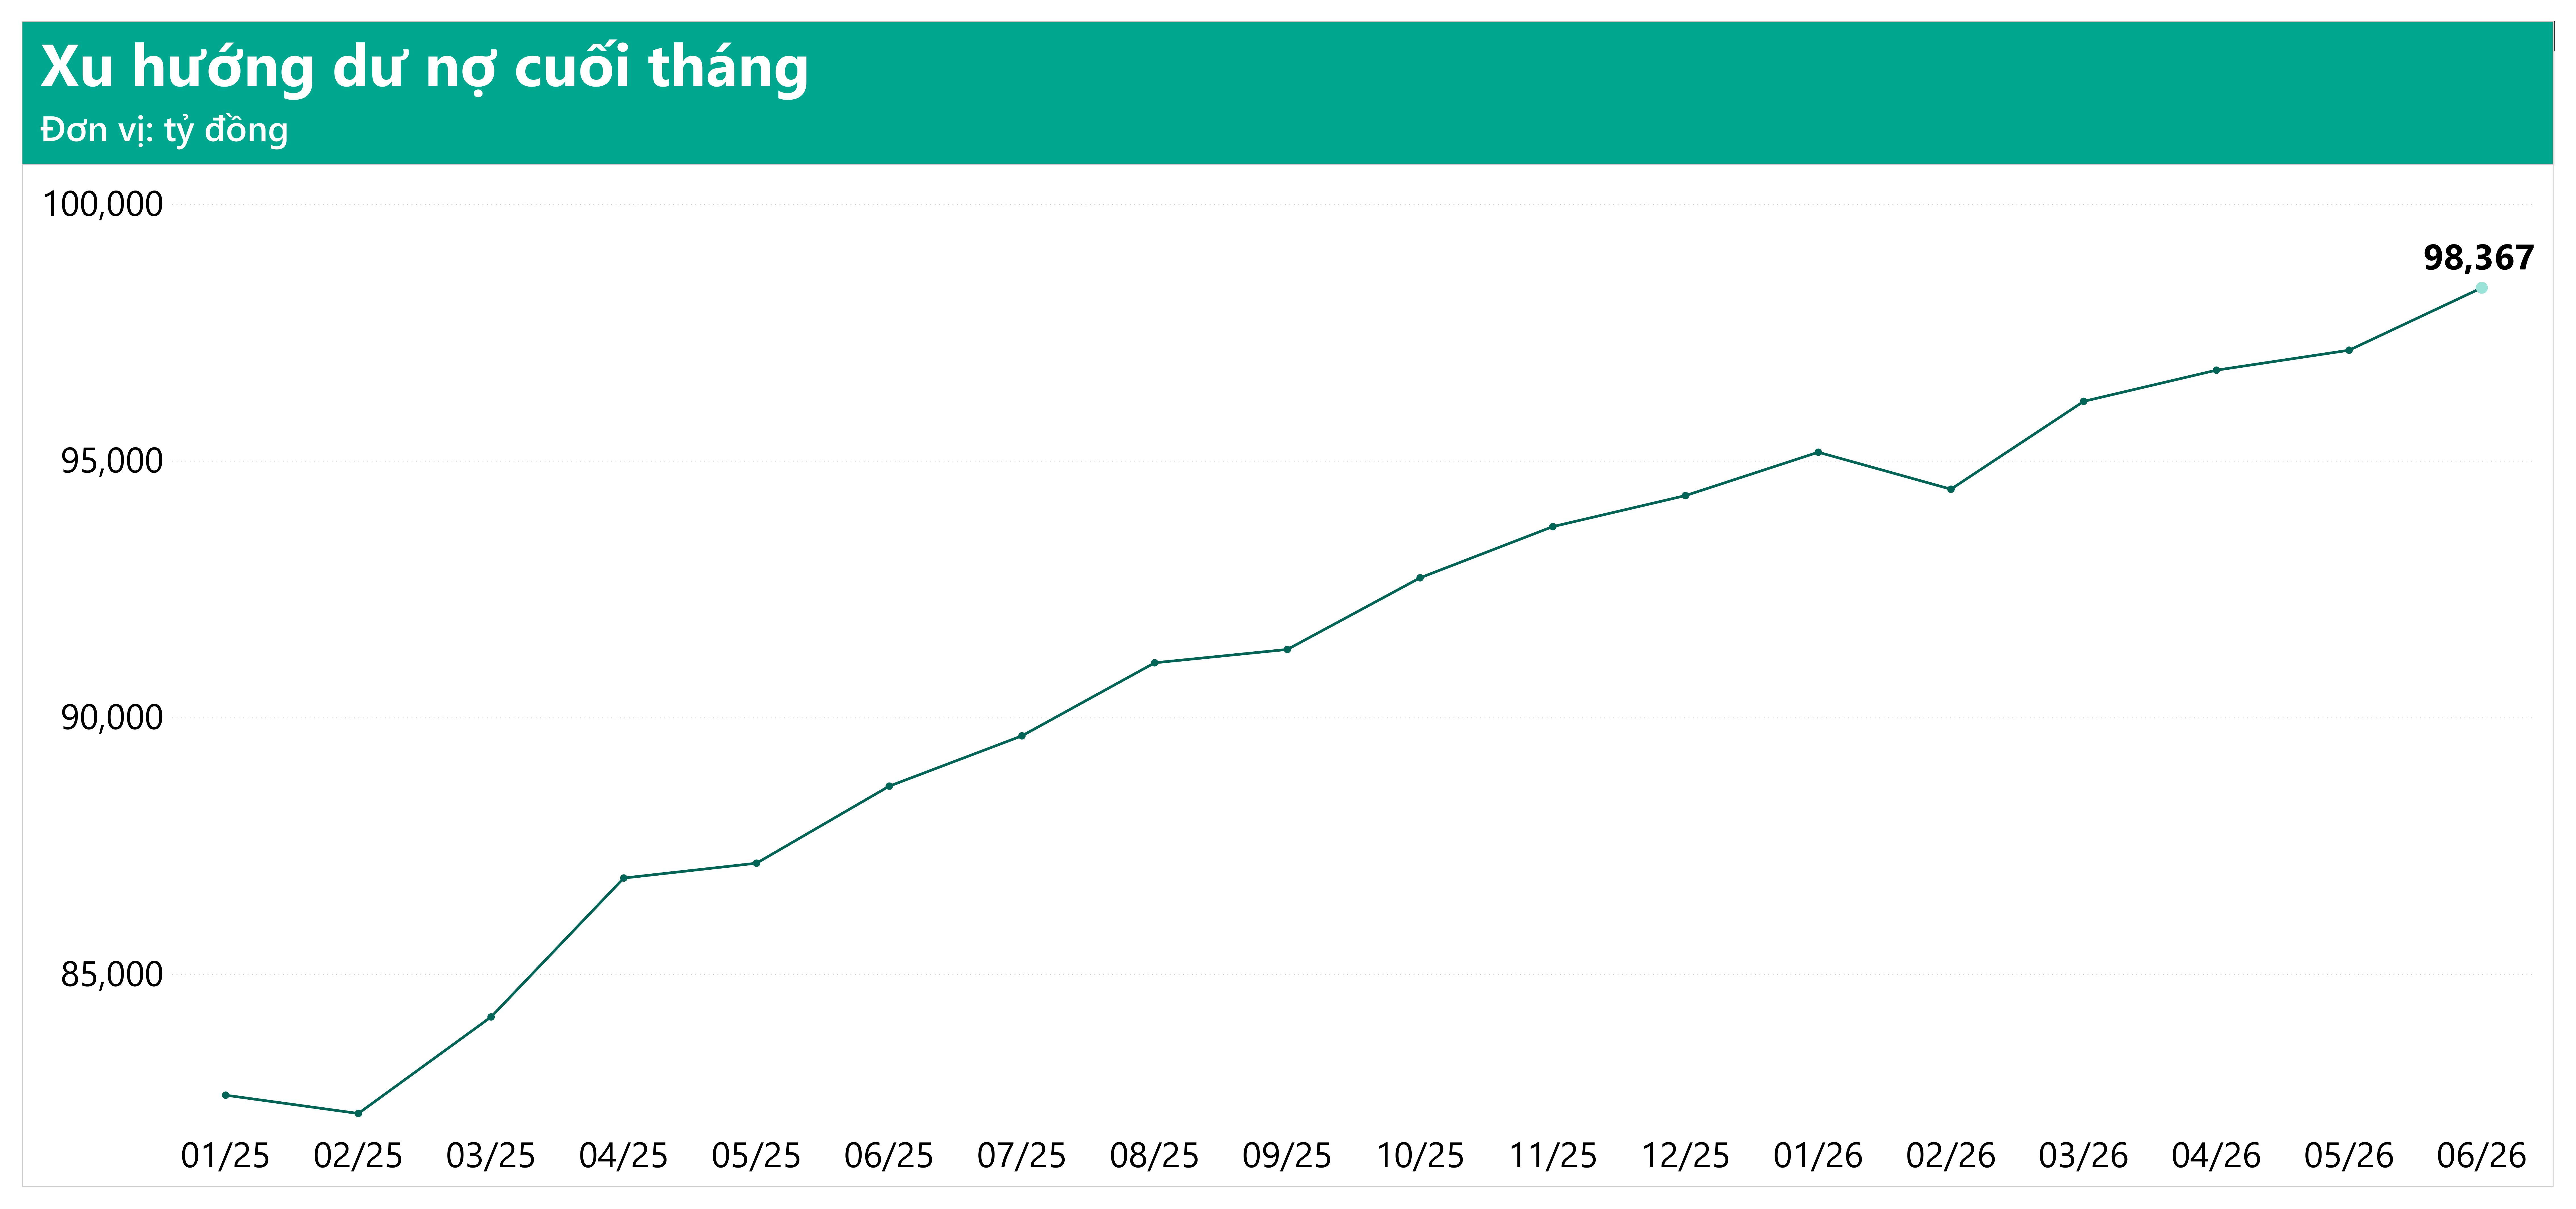
\includegraphics[width=\linewidth]{hinh1.final.jpg}
\caption{Dư nợ cuối tháng tăng từ 82.644 lên 98.367 tỷ đồng trong 18 tháng, chỉ giảm ở tháng 02/2025 và 02/2026. Nguồn: Power BI, giai đoạn 01/2025--06/2026.}
\label{fig:q1-trend}
\end{figure}

\textbf{2. Mức tăng/giảm dư nợ đến từ kỳ hạn, phân khúc, ngành, sản phẩm và ĐVKD nào? Trọng tâm là giá trị tăng tuyệt đối, không chỉ tỷ lệ tăng trưởng?}

Tăng trưởng tháng 6 theo kỳ hạn, phân khúc, ngành và sản phẩm. Theo phép phân rã đóng góp tăng trưởng, dư nợ ST tăng 937,5 tỷ, tương đương 77,1\% mức tăng ròng toàn danh mục. Ở các chiều khác, nhóm đóng góp lớn nhất lần lượt là BIGCORP 1 (+439,8 tỷ; 36,2\%), Công nghiệp \& Xây dựng (+511,1 tỷ; 42,0\%) và CV thường (+1.048,2 tỷ; 86,2\%). Bất động sản giảm 63,7 tỷ, MEDIUM 1 giảm 57,4 tỷ và UPAS X giảm 1,4 tỷ. Các đóng góp theo phân khúc, ngành và sản phẩm cần đối chiếu thêm với Power BI ở cả hai kỳ trước khi chốt. Ở góc ĐVKD, CN Bình Dương 4 là trường hợp lệch pha đáng chú ý: dashboard ghi dư nợ 3.399,6 tỷ, so với 3.089,9 tỷ tháng trước và 3.431,9 tỷ cùng kỳ. Dashboard hiển thị +10,0\% MoM nhưng -0,9\% YoY. Khi đọc cùng YoY, mức tăng trong một tháng cần tiếp tục được theo dõi trước khi kết luận về tăng trưởng dài hạn.

\vspace{0.2cm}

\textbf{3. Top 10 ngành và Top 10 ĐVKD đang chiếm bao nhiêu tổng dư nợ; mức tập trung thay đổi như thế nào qua thời gian?}

Top 10 ĐVKD chiếm 40,10\% tổng dư nợ tại 30/06/2026, tăng 0,24 điểm phần trăm so với tháng trước nhưng giảm 1,33 điểm phần trăm so với cùng kỳ. Top 10 ngành chi tiết chiếm 71,68\%, gần như không đổi so tháng trước và giảm 0,24 điểm phần trăm so với cùng kỳ. Các so sánh này cần xác nhận lại Top 10 được xác định riêng cho từng kỳ; bảng Top 10 hiện tại trên dashboard không tự xác nhận thứ hạng Top 10 của kỳ trước (Hình~\ref{fig:q1-top10}).

\begin{figure}[H]
\centering
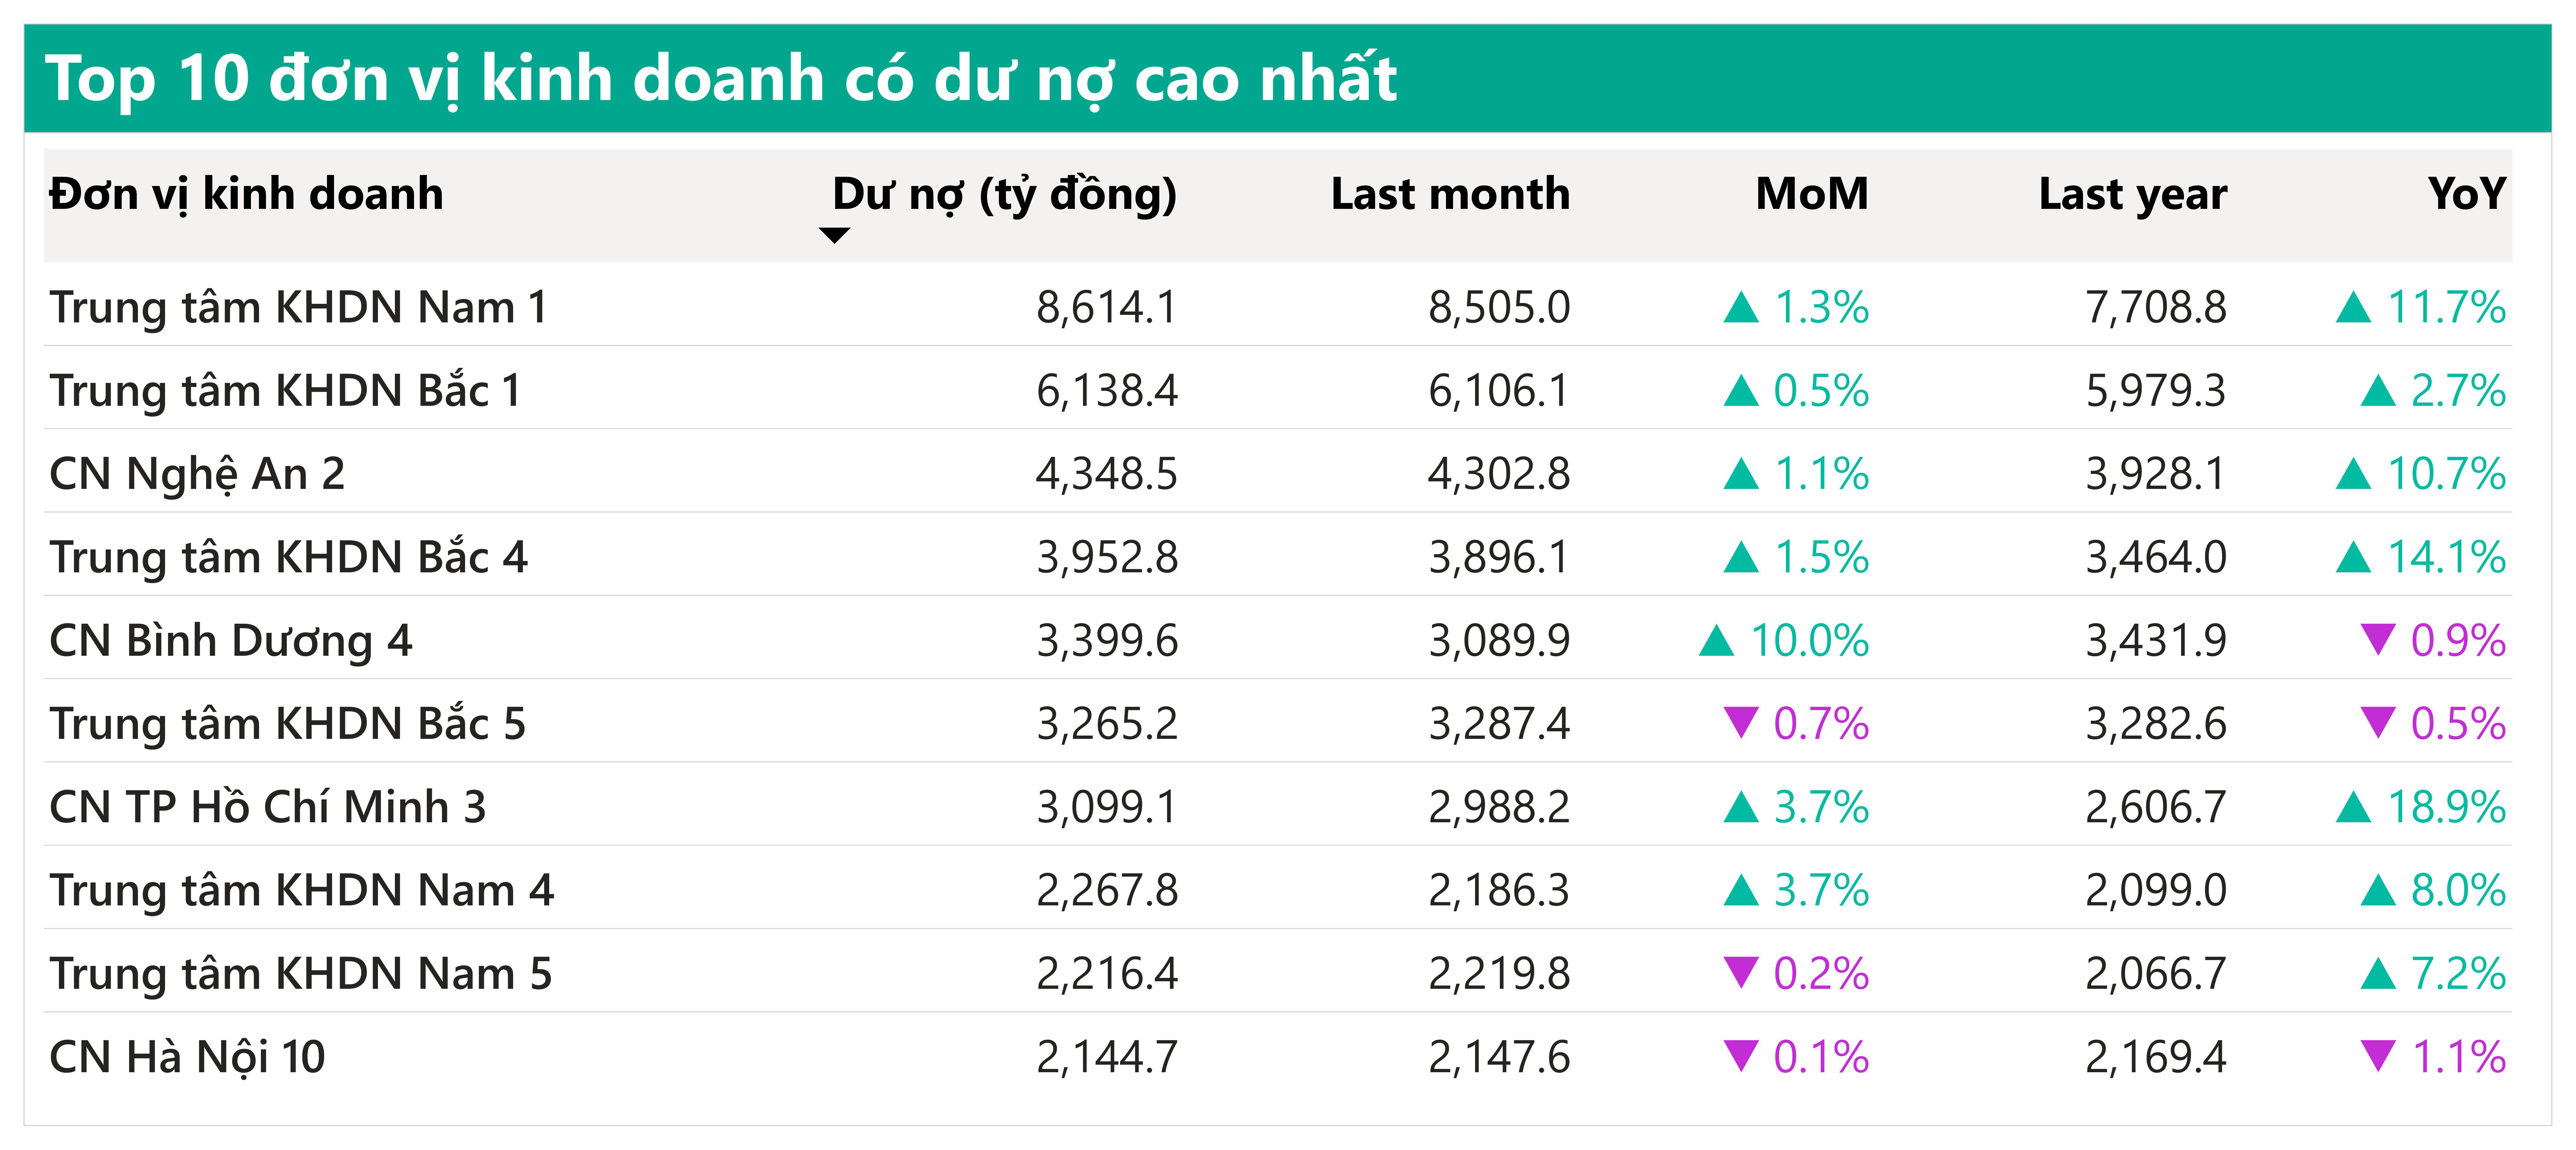
\includegraphics[width=\linewidth]{hinh2.final.jpg}
\caption{Top 10 ĐVKD chiếm 40,10\% tổng dư nợ tại 30/06/2026. CN Bình Dương 4 tăng 10,0\% so với tháng trước nhưng giảm 0,9\% so với cùng kỳ năm trước. Nguồn: Power BI, đơn vị: tỷ đồng.}
\label{fig:q1-top10}
\end{figure}

Ngưỡng P90 lịch sử trong 18 tháng 01/2025–06/2026 là 41,33\% cho Top 10 ĐVKD và 72,01\% cho Top 10 ngành. Trước khi sử dụng làm căn cứ cảnh báo, cần tái lập chuỗi tỷ trọng và đối chiếu cách chọn Top 10, mẫu lịch sử và phương pháp tính P90.

\vspace{0.25cm}

\textbf{Q2: Thu nhập từ danh mục}

\textbf{Trả lời:} Xét theo phân khúc, nguồn thu nhập lãi lớn nhất là nhóm khách hàng quy mô nhỏ (Micro và Small, 50,2\% NII YTD); ở cấp khách hàng đơn lẻ, các khách hàng lớn (BIGCORP 1, UPPER 1) đứng đầu. NII và TOI YTD tăng đều qua các tháng trong năm 2026, nhưng mức tăng khoảng 20\% từ tháng 5 sang tháng 6 chủ yếu do cộng dồn thêm một tháng, nên chưa đủ để kết luận thu nhập tăng tương xứng với dư nợ (xem câu hỏi chi tiết số 2 và Hình~\ref{fig:q2-seg}).

\begin{figure}[H]
\centering

\includegraphics[width=\linewidth]{hinh3.final.jpg}
\caption{Micro và Small chiếm 50,2\% NII YTD (trái), nhưng Top 10 khách hàng có NII lớn nhất không có khách hàng Micro hay Small và chỉ chiếm khoảng 8,2\% NII YTD (phải). Nguồn: Power BI, đến 30/06/2026; đơn vị bảng: tỷ đồng.}
\label{fig:q2-seg}
\end{figure}

\textbf{Dữ liệu cho thấy.}
\begin{itemize}[label=-, leftmargin=0.8cm, itemsep=0.2em]
    \item NII YTD đạt 802,5 tỷ đồng (tăng 19,7\% so với tháng trước) và TOI YTD đạt 1.165,5 tỷ đồng (tăng 20,5\% so với tháng trước).
    \item Phân khúc Micro và Small chiếm 50,2\% tổng NII (Micro: 32,6\%; Small: 17,6\%) và 43,3\% tổng TOI toàn khối KHDN.
    \item Ở cấp khách hàng, 10 khách hàng có NII lớn nhất gồm 4 khách hàng BIGCORP 1 (dẫn đầu là TNHH Xây dựng Vexada, 16,15 tỷ đồng), 3 khách hàng UPPER 1 và 3 khách hàng MEDIUM; không có khách hàng Micro hay Small. Tổng NII của 10 khách hàng này là 65,6 tỷ đồng, khoảng 8,2\% NII YTD.
    \item Về ĐVKD, Trung tâm KHDN Nam 1 (52 tỷ đồng NII) và CN Nghệ An 2 (43 tỷ đồng NII) dẫn đầu hệ thống.
\end{itemize}

\vspace{0.2cm}

\textbf{Nhóm suy luận.} Tỷ trọng NII của MICRO (32,6\%) cao hơn tỷ trọng dư nợ của phân khúc này (20,20\%), trong khi BIGCORP 1 ngược lại (12,3\% NII so với 21,37\% dư nợ). Điều này gợi ý thu nhập lãi trên mỗi đồng dư nợ của Micro cao hơn BIGCORP 1, nhưng cần tính NIM theo phân khúc để xác nhận. Nhóm cũng giả thuyết rằng BIGCORP có thể được giữ vì giá trị bán chéo dịch vụ phi tín dụng, tuy nhiên dữ liệu hiện có chưa kiểm chứng được điều này. Vì Micro và Small là mảng đóng góp NII lớn nhất, cần kiểm tra chéo ở Q3 chất lượng tín dụng của hai phân khúc này.

\vspace{0.2cm}

\subsection*{Trả lời câu hỏi bổ sung (Phân tích chi tiết Q2)}

\textbf{1. Giá trị NII, TOI YTD là bao nhiêu so với cùng kỳ tháng trước?}

Tại thời điểm báo cáo (tháng 06/2026), NII YTD đạt 802,5 tỷ đồng, tăng 19,7\% so với tháng trước. TOI YTD đạt 1.165,5 tỷ đồng, tăng 20,5\% so với tháng trước. Cả hai chỉ tiêu được cộng dồn từ đầu năm và quay về mức đầu kỳ vào tháng 01/2026 (Hình~\ref{fig:q2-trend}).

\begin{figure}[H]
\centering

\includegraphics[width=\linewidth]{hinh4.final.jpg}
\caption{NII YTD (trái) và TOI YTD (phải) tăng đều trong năm 2026, đạt 802,5 và 1.165,5 tỷ đồng ở 06/2026. Số lũy kế đặt lại từ tháng 01 mỗi năm nên mức tăng so với tháng trước luôn dương và không dùng để đánh giá hiệu quả. Đơn vị: tỷ đồng.}
\label{fig:q2-trend}
\end{figure}

\textbf{2. Mức tăng thu nhập có tương xứng với mức tăng dư nợ không?}

Dữ liệu hiện có chưa đủ cơ sở để kết luận. NII và TOI YTD tăng khoảng 20\% từ tháng 5 sang tháng 6 vì đây là chỉ tiêu lũy kế: thu nhập của một tháng được cộng vào tổng của năm tháng trước, tương đương khoảng 1/5, trong khi dư nợ cuối kỳ chỉ tăng 1,25\% MoM. Hai mức tăng này không cùng bản chất nên không so sánh trực tiếp được. Để đánh giá thu nhập có tương xứng với quy mô dư nợ, cần so NII YTD với DNBQ YTD hoặc so với cùng kỳ năm trước.

\vspace{0.2cm}

\textbf{3. Phân khúc, ĐVKD hay nhóm khách hàng nào đang đóng góp trọng yếu?}

Về phân khúc, Micro và Small là nguồn đóng góp lớn nhất, tổng cộng 50,2\% NII YTD (Micro: 32,6\%, Small: 17,6\%). Về khách hàng, nhóm BIGCORP 1 có giá trị tuyệt đối lớn nhất, tiêu biểu là TNHH Xây dựng Vexada (16,15 tỷ đồng). Về ĐVKD, Trung tâm KHDN Nam 1 và CN Nghệ An 2 là hai đơn vị đóng góp lớn nhất (Hình~\ref{fig:q2-branch}).

\begin{figure}[H]
\centering
\includegraphics[width=0.85\linewidth]{hinh5.final.jpg}
\caption{Trung tâm KHDN Nam 1 (52,2 tỷ đồng) và CN Nghệ An 2 (42,7 tỷ đồng) dẫn đầu Top 10 ĐVKD theo NII YTD. Nam 1 chiếm 6,5\% NII YTD toàn khối và 18,5\% tổng NII của Top 10. Nguồn: Power BI, đến 30/06/2026.}
\label{fig:q2-branch}
\end{figure}

\textbf{Q3: Khoản vay có dấu hiệu rủi ro}

\textbf{Trả lời:} Dấu hiệu rủi ro rõ nhất nằm ở nợ xấu OD3-5, tăng 37,8\% so với cùng tháng năm trước, nhanh hơn mức tăng 10,95\% của tổng dư nợ. Mức giảm của dư nợ OD2 không phản ánh chất lượng tín dụng cải thiện, vì chỉ 42\% dư nợ rời OD2 trở về nhóm 1 còn 51\% chuyển sang OD3. Rủi ro của kỳ này tập trung ở một hợp đồng 390 tỷ đồng và ở ba ngành bất động sản, xây lắp, sản xuất điện - điện tử.

\vspace{0.2cm}

\textbf{Trả lời câu hỏi bổ sung (phân tích chi tiết Q3):}

\textbf{1. Tỷ lệ OD2 và OD3-5 hiện tại là bao nhiêu, và đã thay đổi bao nhiêu điểm phần trăm so với cuối tháng trước và cùng tháng năm trước?}

Tỷ lệ OD2 tại 30/06/2026 là 0,94\%, giảm 0,45 điểm phần trăm so với cuối tháng trước nhưng vẫn cao hơn 0,14 điểm phần trăm so với cùng tháng năm trước. Tỷ lệ OD3-5 là 2,63\%, tăng 0,25 điểm phần trăm so với cuối tháng trước và 0,51 điểm phần trăm so với cùng tháng năm trước. Dư nợ OD3-5 tăng 37,8\% so với cùng tháng năm trước, trong khi tổng dư nợ tăng 10,95\%, nên nợ xấu tăng nhanh hơn quy mô danh mục (Bảng~\ref{tab:q3-kpi}). Mức tăng 0,25 điểm phần trăm của tỷ lệ OD3-5 so với cuối tháng trước toàn bộ đến từ một hợp đồng 390 tỷ đồng (Hình~\ref{fig:q3-ratio}), được phân tích thêm ở câu hỏi 3.

\begin{table}[H]
\centering
\caption{Tỷ lệ OD2 giảm so với cuối tháng trước nhưng cao hơn cùng tháng năm trước, còn tỷ lệ OD3-5 tăng ở cả hai mốc so sánh. Nguồn: dashboard, trang CLTD, 30/06/2026.}
\label{tab:q3-kpi}
\vspace{0.15cm}
\renewcommand{\arraystretch}{1.6}
\begin{tabularx}{0.95\linewidth}{@{} 
    >{\raggedright\arraybackslash\bfseries}X 
    >{\centering\arraybackslash}p{2.8cm} 
    >{\centering\arraybackslash}p{3.8cm} 
    >{\centering\arraybackslash}p{4cm} @{}}
  \toprule
  \textit{Chỉ tiêu} & \textit{30/06/2026} & \textit{So với cuối tháng trước} & \textit{So với cùng tháng năm trước} \\
  \midrule
  Tỷ lệ OD2 & 0,94\% & $-0{,}45$ điểm \% & $+0{,}14$ điểm \% \\
  Tỷ lệ OD3-5 & 2,63\% & $+0{,}25$ điểm \% & $+0{,}51$ điểm \% \\
  Dư nợ OD2 & 927,5 tỷ đồng & $-31{,}6\%$ & $+29{,}8\%$ \\
  Dư nợ OD3-5 & 2.586,5 tỷ đồng & $+11{,}7\%$ & $+37{,}8\%$ \\
  \bottomrule
\end{tabularx}
\end{table}

\begin{figure}[H]
\centering
\includegraphics[width=0.75\linewidth]{hinh8.final.jpg}
\caption{Một hợp đồng 390 tỷ đồng tạo ra toàn bộ mức tăng 0,25 điểm phần trăm của tỷ lệ OD3-5. Khi loại hợp đồng này, tỷ lệ giảm 0,14 điểm phần trăm so với cuối tháng trước. Giá trị 2,24\% là ước tính của nhóm từ dư nợ OD3-5 và tổng dư nợ ngày 30/06/2026.}
\label{fig:q3-ratio}
\end{figure}

% TODO (Người 3): thêm bảng hoặc hình OD3-5 theo phân khúc (kèm tỷ trọng dư nợ), dòng vào OD2 theo ngành và ĐVKD từ trang CLTD.
\textbf{2. Rủi ro tập trung ở ngành, đơn vị kinh doanh (ĐVKD) và phân khúc nào?}

Về mức độ tập trung, ba ngành bất động sản (520 tỷ đồng, 20,1\%), xây lắp (413 tỷ đồng, 16,0\%) và sản xuất điện - điện tử (397 tỷ đồng, 15,4\%) chiếm tổng cộng 51,4\% dư nợ OD3-5 (Hình~\ref{fig:q3-conc}). Trung tâm KHDN Bắc 1 có 549 tỷ đồng, tương đương 21,2\% dư nợ OD3-5 của toàn ngân hàng, và 71\% số đó là hợp đồng AIV-LN-0007842 (phân tích ở câu hỏi 3). Dư nợ OD3-5 có ở 73 ĐVKD, và năm ĐVKD đứng đầu, kể cả Bắc 1, chiếm 38,9\%. Theo phân khúc, MICRO (610 tỷ đồng, 23,6\%) và SMALL (555 tỷ đồng, 21,5\%) có dư nợ OD3-5 lớn nhất; riêng MICRO chiếm 23,6\% dư nợ OD3-5 so với 20,20\% tổng dư nợ, tức nợ xấu của MICRO cao hơn tỷ trọng quy mô. Nợ nhóm 5 chiếm 43,8\% dư nợ OD3-5 (1.132,9 tỷ đồng, 187 hợp đồng). Xây lắp cũng là ngành có dòng nợ đi vào OD2 từ nhóm 1 lớn nhất, với 218 tỷ đồng, tương đương 39\% dòng này.

\begin{figure}[H]
\centering

\includegraphics[width=\linewidth]{hinh6.final.jpg}
\caption{Ba ngành chiếm 51,4\% dư nợ OD3-5 (trái). Trung tâm KHDN Bắc 1 chiếm 21,2\% (549 tỷ đồng), gồm 159 tỷ đồng từ các hợp đồng còn lại (phần xanh) và 390 tỷ đồng từ hợp đồng AIV-LN-0007842 (phần tím), tức hợp đồng này nằm trong 549 tỷ đồng và không cộng thêm (phải). Tỷ trọng tính trên dư nợ OD3-5 tại 30/06/2026, chưa phải tỷ lệ nợ xấu của từng ngành hay ĐVKD.}
\label{fig:q3-conc}
\end{figure}

\textbf{3. Khi dư nợ OD2 giảm, phần giảm đến từ khoản vay trở về nhóm 1 hay từ khoản vay chuyển sang nhóm nợ xấu hơn?}

Dư nợ OD2 giảm 429 tỷ đồng, từ 1.356,6 tỷ đồng ở 31/05 xuống 927,5 tỷ đồng ở 30/06, nhưng mức giảm này là kết quả của hai dòng ngược chiều (Hình~\ref{fig:q3-od2}). Trong 1.013 tỷ đồng rời OD2, 424 tỷ đồng (42\%) trở về nhóm 1, 514 tỷ đồng (51\%) chuyển sang OD3 và 74 tỷ đồng (7\%) ra khỏi dư nợ. Cùng kỳ, 594 tỷ đồng đi vào OD2, gồm 563 tỷ đồng từ nhóm 1 và 31 tỷ đồng từ bốn hợp đồng mới. Vì vậy, chỉ 424 tỷ đồng, tương đương 31\% dư nợ OD2 đầu kỳ, thực sự trở về nhóm 1, và chỉ 36\% dư nợ OD2 cuối kỳ (333 tỷ đồng) là khoản đã nằm trong OD2 từ cuối tháng trước. Mức giảm 31,6\% của dư nợ OD2 vì thế chưa đủ để kết luận chất lượng tín dụng cải thiện.

\begin{figure}[H]
\centering
\includegraphics[width=0.85\linewidth]{hinh7.final.jpg}
\caption{Dư nợ OD2 giảm 429 tỷ đồng, nhưng chỉ 424 tỷ đồng trở về nhóm 1, trong khi 514 tỷ đồng chuyển sang OD3 và 594 tỷ đồng mới đi vào OD2. Đơn vị: tỷ đồng. Màu xanh đậm là dư nợ OD2 tại hai mốc, màu xanh ngọc là dòng trở về nhóm 1, màu tím là dòng làm tăng rủi ro (chuyển sang OD3, vào từ nhóm 1, hợp đồng mới), màu xám là dòng còn lại.}
\label{fig:q3-od2}
\end{figure}

Một hợp đồng quyết định phần lớn dòng chuyển sang OD3. Hợp đồng AIV-LN-0007842 có dư nợ 390 tỷ đồng, thuộc phân khúc BIGCORP 1, ngành sản xuất điện - điện tử, do Trung tâm KHDN Bắc 1 hạch toán và quá hạn 96 ngày. Hợp đồng này chiếm 76\% dòng OD2 sang OD3. Nếu loại ra, dòng này chỉ còn 122 tỷ đồng ở 25 hợp đồng. Khi loại hợp đồng này khỏi cả dư nợ OD3-5 và tổng dư nợ, tỷ lệ OD3-5 ước tính là 2,24\%, thấp hơn 0,14 điểm phần trăm so với mức 2,38\% của cuối tháng trước (Hình~\ref{fig:q3-ratio}). Mức tăng 0,25 điểm phần trăm trên dashboard do đó đến toàn bộ từ một hợp đồng. Hợp đồng này cũng giải thích phần lớn biến động của Trung tâm KHDN Bắc 1, nơi tỷ lệ OD2 giảm từ 6,68\% xuống 1,24\% và tỷ lệ OD3-5 tăng từ 2,37\% lên 8,94\%, vì 390 tỷ đồng tương đương 6,35 điểm phần trăm trên tổng dư nợ 6.138,4 tỷ đồng của đơn vị này.

\section{Tổng hợp phát hiện}

Với mỗi phát hiện, nhóm tách điều dữ liệu cho thấy khỏi điều nhóm suy luận thêm, và ghi rõ phần nào còn cần kiểm tra.

\begin{enumerate}[label=\textbf{\arabic*.}, leftmargin=0.8cm]

\item \textbf{Quy mô tiếp tục mở rộng.}\\
    \textit{Finding:} Dư nợ 30/06/2026 đạt 98.367,3 tỷ VND, tăng 1.215,8 tỷ (+1,25\% MoM) và 9.705,2 tỷ (+10,95\% YoY). DNBQ YTD đạt 96.004,0 tỷ, tăng 0,4\% MoM và 13,3\% YoY theo Power BI.\\
    \textit{Insight:} Tăng trưởng hiện tại chủ yếu được dẫn dắt bởi danh mục cốt lõi – dư nợ ngắn hạn và CV thường – thay vì các sản phẩm quy mô nhỏ. Cần xác nhận thêm đóng góp theo sản phẩm trên dashboard.

\item \textbf{Tăng trưởng có nguồn kéo khá rõ.}\\
    \textit{Finding:} ST đóng góp 77,1\% mức tăng MoM; CV thường đóng góp 86,2\%. BIGCORP 1 (+439,8 tỷ) và Công nghiệp \& Xây dựng (+511,1 tỷ) là hai nguồn tăng nổi bật. CN Bình Dương 4 tăng MoM nhưng vẫn giảm YoY. Các đóng góp theo phân khúc, ngành và sản phẩm cần đối chiếu thêm trên Power BI.\\
    \textit{Insight:} CN Bình Dương 4 minh họa rủi ro khi chỉ đọc MoM: tăng mạnh trong tháng nhưng vẫn thấp hơn cùng kỳ. Cần dùng đồng thời MoM và YoY khi theo dõi các ĐVKD biến động lớn.

\item \textbf{Tập trung không xấu đi rõ rệt.}\\
    \textit{Finding:} Top 10 ĐVKD chiếm 40,10\%, giảm 1,33 điểm phần trăm YoY; Top 10 ngành chiếm 71,68\%, gần như đi ngang MoM và giảm 0,24 điểm phần trăm YoY. Hai chỉ số dưới ngưỡng P90 lịch sử 18 tháng. Cần tái lập các kết quả trước khi kết luận.\\
    \textit{Insight:} Quy mô tăng nhưng mức tập trung theo ĐVKD không tăng theo cùng tốc độ. Kết luận này phụ thuộc vào việc xác định đúng Top 10 ở từng kỳ.

% TODO (Người 2): thay "so với tháng trước" bằng NII/TOI YTD 6T/2026 so với 6T/2025 lấy từ dashboard, so với tăng dư nợ YoY 10,95\%.
\item \textbf{Phân cực nguồn thu: Micro/Small gánh vác tỷ trọng chính, BIGCORP thống trị giá trị tuyệt đối.}\\
    \textit{Finding:} NII YTD đạt 802,5 tỷ và TOI YTD đạt 1.165,5 tỷ (đều tăng xấp xỉ 20\% so với tháng trước). Phân khúc Micro và Small chiếm hơn nửa (50,2\%) tổng NII toàn khối. Trái lại, Top 10 khách hàng có NII lớn nhất không có khách hàng Micro hay Small (4 BIGCORP 1, 3 UPPER 1, 3 MEDIUM; dẫn đầu mang về 16,15 tỷ) và chỉ chiếm khoảng 8,2\% NII YTD.\\
    \textit{Insight:} Nguồn thu lãi dựa vào số đông khách hàng quy mô nhỏ hơn là một vài khách hàng lớn. Tỷ trọng NII của MICRO (32,6\%) cao hơn tỷ trọng dư nợ (20,20\%), còn BIGCORP 1 thấp hơn (12,3\% so với 21,37\%), gợi ý thu nhập lãi trên mỗi đồng dư nợ của Micro cao hơn; cần tính NIM theo phân khúc để xác nhận.

\item \textbf{Dư nợ OD2 giảm không đồng nghĩa chất lượng tín dụng cải thiện; rủi ro tập trung vào một khoản lớn.}\\
    \textit{Finding:} Dư nợ OD2 giảm 31,6\% so với cuối tháng trước, từ 1.356,6 tỷ đồng xuống 927,5 tỷ đồng, nhưng trong 1.013 tỷ đồng rời OD2 chỉ 42\% trở về nhóm 1 và 51\% chuyển sang OD3. Dư nợ OD3-5 tăng 11,7\% so với cuối tháng trước và 37,8\% so với cùng tháng năm trước, nhanh hơn mức tăng 10,95\% của tổng dư nợ. Một hợp đồng 390 tỷ đồng chiếm 76\% dòng OD2 sang OD3. Khi loại hợp đồng này, tỷ lệ OD3-5 ước tính giảm 0,14 điểm phần trăm thay vì tăng 0,25 điểm phần trăm. Ba ngành bất động sản, xây lắp và sản xuất điện - điện tử chiếm 51,4\% dư nợ OD3-5, và Trung tâm KHDN Bắc 1 chiếm 21,2\%. MICRO chiếm 23,6\% dư nợ OD3-5, cao hơn tỷ trọng 20,20\% trong tổng dư nợ.\\
    \textit{Insight:} Mức giảm của OD2 trên dashboard chưa cho thấy chất lượng tín dụng cải thiện, vì phần lớn dòng rời OD2 chuyển sang nhóm nợ xấu hơn và nợ mới vẫn liên tục đi vào OD2. Rủi ro của kỳ này tập trung vào một khoản lớn, khoản này quyết định bức tranh tỷ lệ chung. Phần nền của nợ xấu là nợ nhóm 5, gần như không đổi nhóm trong kỳ và nằm ở một số ngành.

\end{enumerate}

\section{Đề xuất}

Các đề xuất được xếp theo thứ tự nên làm. Với những việc mà nguyên nhân chưa rõ, nhóm đề xuất kiểm tra hoặc thử nghiệm trước khi thay đổi lớn.

\vspace{0.3cm}
\textbf{Làm ngay}
\vspace{0.1cm}
\hrule
\vspace{0.3cm}

\begin{itemize}[label=--, leftmargin=0.8cm]
    
    \item \textbf{Giữ nền tảng Micro và Small nhưng gắn với theo dõi chất lượng tín dụng của hai phân khúc này; xem xét bán chéo cho nhóm BIGCORP.}\\
    \textit{Căn cứ:} Micro và Small đóng góp 50,2\% tổng NII toàn khối, nhưng MICRO cũng chiếm 23,6\% dư nợ OD3-5, cao hơn tỷ trọng 20,20\% trong tổng dư nợ (Phát hiện 4 và 5). BIGCORP 1 có tỷ trọng NII (12,3\%) thấp hơn tỷ trọng dư nợ (21,37\%).\\
    \textit{Theo dõi bằng:} NIM và tỷ lệ OD3-5 tách theo từng phân khúc; tỷ trọng đóng góp NII và TOI của các nhóm.

    \item \textbf{Lập danh sách theo dõi các khoản lớn.}\\
    Đưa vào danh sách theo dõi riêng những khoản có dư nợ lớn đang ở OD2 hoặc quá hạn từ 60 ngày (ngưỡng đề xuất), bắt đầu từ hợp đồng AIV-LN-0007842 và các khoản lớn khác trong 26 hợp đồng đã chuyển sang OD3.\\
    \textit{Căn cứ:} Một hợp đồng đơn lẻ đã chiếm tới 76\% dòng chuyển từ OD2 sang OD3.\\
    \textit{Theo dõi bằng:} Số lượng khoản vay và tổng dư nợ trong danh sách này, cùng số khoản chuyển nhóm mỗi tháng.

    \item \textbf{Báo cáo tỷ lệ OD3-5 kèm tỷ lệ khi loại trừ khoản lớn nhất.}\\
    Nên báo cáo riêng khi một khoản đơn lẻ làm tỷ lệ lệch hơn 0,10 điểm phần trăm (ngưỡng đề xuất).\\
    \textit{Căn cứ:} Hợp đồng 390 tỷ đồng đã làm tỷ lệ OD3-5 lệch 0,39 điểm phần trăm trên tổng dư nợ, làm sai lệch bức tranh rủi ro chung.\\
    \textit{Theo dõi bằng:} Báo cáo so sánh tỷ lệ thực tế và tỷ lệ điều chỉnh.
    
    \item \textbf{Theo dõi hằng tháng dòng chuyển nhóm từ OD2.}\\
    Ngưỡng cảnh báo cần được chốt sau khi xem xét thêm xu hướng các tháng trước.\\
    \textit{Căn cứ:} Cần kiểm soát mức độ trượt nhóm. Tháng này 38\% dư nợ OD2 đầu kỳ chuyển sang OD3 (còn 13\% nếu loại hợp đồng 390 tỷ) và 31\% trở về nhóm 1.\\
    \textit{Theo dõi bằng:} Chỉ số phần dư nợ OD2 đầu kỳ chuyển sang OD3 và phần trở về nhóm 1.

\end{itemize}

\vspace{0.3cm}
\textbf{Rà soát thêm}
\vspace{0.1cm}
\hrule
\vspace{0.3cm}

\begin{itemize}[label=--, leftmargin=0.8cm]

    \item \textbf{Ưu tiên rà soát rủi ro theo ngành và ĐVKD.}\\
    Rà soát sớm ngành xây lắp, sau đó đến bất động sản và sản xuất điện - điện tử. Về ĐVKD, ưu tiên Trung tâm KHDN Nam 1 và Trung tâm KHDN Bắc 1.\\
    \textit{Căn cứ:} Ngành xây lắp vừa nằm trong top 3 dư nợ OD3-5 lớn nhất vừa có dòng đi vào OD2 cao nhất. Trung tâm KHDN Nam 1 có dòng đi vào OD2 từ nhóm 1 cao nhất (102 tỷ), và Bắc 1 có dư nợ OD3-5 lớn nhất.\\
    \textit{Theo dõi bằng:} Tỷ trọng ba ngành này trong dư nợ OD3-5 và dòng đi vào OD2 phân tách theo từng ngành.

    \item \textbf{Xác nhận lý do nợ nhóm 5 ra khỏi dư nợ.}\\
    Chỉ được tính là có sự cải thiện thực chất khi nguyên nhân là thu hồi nợ thành công, không tính các khoản xóa nợ.\\
    \textit{Căn cứ:} Có khoản 163 tỷ đồng nợ nhóm 5 (11 hợp đồng) vừa ra khỏi dư nợ.\\
    \textit{Theo dõi bằng:} Tỷ lệ thu hồi trên tổng số nợ nhóm 5 ra khỏi dư nợ.

\end{itemize}

\section{Hạn chế và bước tiếp theo}

\begin{enumerate}[label=\textbf{\arabic*.}, leftmargin=0.8cm]

    \item \textbf{Phân tích dư nợ và mức tập trung.}\\
    Dữ liệu số dư chỉ có tại cuối tháng, nên phân tích xác định được chênh lệch giữa hai snapshot nhưng không quan sát trực tiếp các dòng giải ngân, thu nợ, tất toán hay tái tục trong tháng. Vì vậy chưa đủ cơ sở kết luận nguyên nhân nghiệp vụ tạo ra thay đổi số dư.\\
    \textit{Bước tiếp theo:} Bổ sung dữ liệu giao dịch hoặc snapshot theo ngày/tuần để giải thích biến động lớn như CN Bình Dương 4. Với chỉ số tập trung, tái lập Top 10 ở từng kỳ, kiểm tra P90/P95 và đối chiếu với khẩu vị rủi ro trước khi dùng làm ngưỡng quản trị.

    \item \textbf{ĐVKD hạch toán khác với ĐVKD quản lý khách hàng.}\\
    Dữ liệu NII/TOI hiện tại được ghi nhận theo đơn vị hạch toán khoản vay. Điều này có thể làm sai lệch bức tranh đánh giá hiệu quả kinh doanh thực tế, đặc biệt với nhóm khách hàng lớn (BIGCORP) thường do Hội sở quản lý nhưng lại giải ngân tại chi nhánh.\\
    \textit{Bước tiếp theo:} trích xuất thêm trường dữ liệu ``ĐVKD quản lý'' từ hệ thống CRM để đối chiếu và phân bổ lại thu nhập cho chính xác.

    \item \textbf{Đánh giá rủi ro tín dụng.}\\
    Dữ liệu chỉ ghi số dư cuối tháng, nên phân tích không thấy được khoản vay trượt nhóm rồi quay lại ngay trong tháng, và dòng chuyển nhóm giữa 31/05 và 30/06/2026 mới phản ánh một tháng, chưa đủ để kết luận xu hướng. Bảng hợp đồng chỉ gồm khoản có nhóm nợ từ 2 trở lên ở ít nhất một mốc, nên tỷ trọng theo ngành và ĐVKD là tỷ trọng trong dư nợ OD3-5, chưa phải tỷ lệ nợ xấu của từng ngành hay ĐVKD. Dữ liệu chưa ghi lý do ra khỏi dư nợ của 21 hợp đồng (274 tỷ đồng), nên chưa xác định được các khoản này được thu hồi hay xóa nợ.\\
    \textit{Bước tiếp theo:} Bổ sung số dư các tháng trước để kiểm tra mức chuyển nhóm OD2 sang OD3 và tỷ lệ trở về nhóm 1 có ổn định theo thời gian hay không. Bổ sung lý do ra khỏi dư nợ của 21 hợp đồng để phân biệt thu hồi với xóa nợ. Tính dư nợ tổng theo ngành và ĐVKD để chuyển tỷ trọng thành tỷ lệ nợ xấu.

\end{enumerate}

\section{Tài liệu tham khảo}

\begin{enumerate}[label={[\arabic*]}, leftmargin=0.8cm]

    \item AI VIET NAM. ``Corporate Banking Analytics -- Quy trình phân tích dữ liệu tín dụng: Từ câu hỏi kinh doanh đến bộ chỉ số (KPIs), báo cáo trực quan, phân tích và đề xuất hành động''. Tài liệu mô tả project, AI VIET NAM -- End-to-End Data Analytics (eDA). [Online]. Available: \url{https://eda.aivietnam.edu.vn/}

    \item AI VIET NAM. ``eDA Conquer 2026 -- Corporate Banking Dataset''. Dữ liệu đã ẩn danh, đơn vị tiền quy ước, AI VIET NAM -- End-to-End Data Analytics (eDA). [Online]. Available: \url{https://drive.google.com/drive/folders/1wWKVXdnNdkfR7F1XSeqvoINo2em28rJ-?usp=drive_link}

\end{enumerate}

\begin{appendices}

Phụ lục chứa các nội dung dùng để kiểm tra và tái lập phân tích, không nằm trong mạch chính của báo cáo.

\subsection*{A. Dashboard và dữ liệu}

\begin{itemize}[label=--, leftmargin=0.8cm, itemsep=0.2em]
    \item \textbf{File Power BI:} \textit{Datalyst\_Conquer\_Mod2\_Dashboard\_v1}. Các hình 1 đến 8 và Bảng 1 đều lấy từ file này.
    \item \textbf{Data dictionary:} theo tài liệu mô tả bảng và trường dữ liệu của đề bài.
    \item \textbf{Repository GitHub của nhóm:} \url{https://github.com/AIVIETNAM-AIO-kiennguyen210/eda-conquer-mod2-2026-datalyst}. Repository chứa dữ liệu (\texttt{data/}), file Power BI (\texttt{dashboard/}), slide (\texttt{slides/}) và mã nguồn báo cáo (\texttt{report/}).
\end{itemize}

\subsection*{B. Định nghĩa chỉ tiêu và dòng chuyển nhóm}

\begin{table}[H]
\centering
\caption{Định nghĩa tỷ lệ OD và sáu thành phần dòng chuyển nhóm OD2 giữa 31/05 và 30/06/2026 (Hình~\ref{fig:q3-od2}).}
\vspace{0.15cm}
\renewcommand{\arraystretch}{1.6}
\begin{tabularx}{0.95\linewidth}{@{}
    >{\raggedright\arraybackslash\bfseries}p{4.4cm}
    >{\raggedright\arraybackslash}X @{}}
  \toprule
  \textbf{Chỉ tiêu} & \textbf{Ý nghĩa hoặc công thức} \\
  \midrule
  Tỷ lệ OD2, OD3-5 & Dư nợ của nhóm chia cho tổng dư nợ cuối tháng. Thay đổi của tỷ lệ tính bằng điểm phần trăm, là hiệu số hai tỷ lệ. \\
  Tỷ lệ OD3-5 khi loại một hợp đồng & (OD3-5 $-$ dư nợ hợp đồng) chia (tổng dư nợ $-$ dư nợ hợp đồng), cùng ngày. \\
  Về nhóm 1 & Hợp đồng ở OD2 ngày 31/05 và ở nhóm 1 ngày 30/06. \\
  Sang OD3 & Hợp đồng ở OD2 ngày 31/05 và ở nhóm 3 trở lên ngày 30/06. \\
  Ra khỏi dư nợ & Hợp đồng ở OD2 ngày 31/05 và không còn số dư ngày 30/06. \\
  Vào từ nhóm 1 & Hợp đồng ở nhóm 1 ngày 31/05 và ở OD2 ngày 30/06. \\
  Hợp đồng mới & Hợp đồng chưa có số dư ngày 31/05 và ở OD2 ngày 30/06. \\
  Biến động hợp đồng còn lại & Thay đổi số dư của hợp đồng ở OD2 cả hai ngày. \\
  \bottomrule
\end{tabularx}
\end{table}

Tổng sáu thành phần dòng chuyển nhóm cộng với OD2 ngày 31/05 (1.356,6 tỷ đồng) bằng OD2 ngày 30/06 (927,5 tỷ đồng).

\subsection*{C. Kiểm tra độ nhạy khi loại hợp đồng AIV-LN-0007842}

\begin{table}[H]
\centering
\caption{Khi loại hợp đồng 390 tỷ đồng, tỷ lệ OD3-5 toàn ngân hàng giảm từ 2,63\% xuống 2,24\% và tỷ lệ của Trung tâm KHDN Bắc 1 giảm từ 8,94\% xuống 2,77\%. Nguồn: dashboard trang CLTD và tính toán của nhóm, 30/06/2026.}
\vspace{0.15cm}
\renewcommand{\arraystretch}{1.6}
\begin{tabularx}{0.95\linewidth}{@{}
    >{\raggedright\arraybackslash\bfseries}X
    >{\centering\arraybackslash}p{3cm}
    >{\centering\arraybackslash}p{3.6cm} @{}}
  \toprule
  \textbf{Chỉ tiêu} & \textbf{Số thực tế} & \textbf{Khi loại hợp đồng} \\
  \midrule
  Tỷ lệ OD3-5, toàn ngân hàng & 2,63\% & 2,24\% \\
  Thay đổi so với cuối tháng trước (2,38\%) & $+0{,}25$ điểm \% & $-0{,}14$ điểm \% \\
  Tỷ lệ OD3-5, Trung tâm KHDN Bắc 1 & 8,94\% & 2,77\% \\
  Phần OD2 đầu kỳ chuyển sang OD3 & 38\% & 13\% \\
  \bottomrule
\end{tabularx}
\end{table}

Ghi chú. Mốc 2,38\% của cuối tháng trước chưa trừ số dư hợp đồng khỏi tổng dư nợ, chênh lệch so với cách tính cùng cơ sở khoảng 0,01 điểm phần trăm và không đổi kết luận. Tỷ lệ 13\% tính bằng (514 $-$ 390) chia (1.356,6 $-$ 390), tức mẫu số cũng đã loại hợp đồng.

\end{appendices}

\end{document}
